\documentclass[11pt,a4paper]{article}

\usepackage[font=small,labelfont=bf,margin=0mm,labelsep=period,tableposition=top]{caption}
\usepackage[a4paper,top=1.5cm,bottom=1.5cm,left=1.5cm,right=1.5cm,bindingoffset=0mm]{geometry}

\usepackage{graphicx}
\usepackage{hyperref}

\usepackage{amsmath} % for aligned
%\usepackage{amssymb} % for \mathbb
\usepackage{tikz}
%\usepackage{etoolbox} % for \ifthen
\usepackage{listofitems} % for \readlist to create arrays
\usetikzlibrary{arrows.meta} % for arrow size
\usepackage[outline]{contour} % glow around text
\contourlength{1.4pt}

\tikzset{>=latex} % for LaTeX arrow head
\usepackage{xcolor}
\colorlet{myred}{red!80!black}
\colorlet{myblue}{blue!80!black}
\colorlet{mygreen}{green!60!black}
\colorlet{myorange}{orange!70!red!60!black}
\colorlet{mydarkred}{red!30!black}
\colorlet{mydarkblue}{blue!40!black}
\colorlet{mydarkgreen}{green!30!black}
\tikzstyle{node}=[thick,circle,draw=black,minimum size=22,inner sep=0.5,outer sep=0.6]
\tikzstyle{node in}=[node]
\tikzstyle{node hidden}=[node]
\tikzstyle{node out}=[node]
\tikzstyle{connect}=[thick] %,line cap=round
\tikzstyle{connect arrow}=[-{Latex[length=4,width=3.5]},thick,shorten <=0.5,shorten >=1]
\tikzset{ % node styles, numbered for easy mapping with \nstyle
  node 1/.style={node in},
  node 2/.style={node hidden},
  node 3/.style={node out},
}
\def\nstyle{int(\lay<\Nnodlen?min(2,\lay):3)} % map layer number onto 1, 2, or 3




\begin{document}
\vspace{-2.0cm}
\begin{flushright}
  Edinburgh 20xx/xx
\end{flushright}
\vspace{0.3cm}

\begin{center}
  {\Large \bf From Field Theory to the mathematics of Deep Learning}\\
  \vspace{1.1cm}
  {\small
    Luigi Del Debbio and Roy Stegeman
  }\\

  \vspace{0.7cm}

  {\it \small
  ~The Higgs Centre for Theoretical Physics, University of Edinburgh,\\
  JCMB, KB, Mayfield Rd, Edinburgh EH9 3JZ, Scotland
  }

  \vspace{1.0cm}

  {\bf \large Abstract}
\end{center}

Abstract

\clearpage

\tableofcontents


\section{Introduction}
In this note we summarize the current understanding of neural networks using an effective field theory approach based on Ref.~\cite{Roberts:2021fes}. We aim to extend the work in Ref.~\cite{Roberts:2021fes} by constructing a more general theory for the training of neural networks based on gradient descent algorithms with regulation based on a training/validation split and early stopping algorithm, thereby providing a theoretical framework for the algorithm used in by the NNPDF collaboration~\cite{NNPDF:2021njg}.


\section{Neural Networks}


\begin{figure}
  \centering
  % NEURAL NETWORK with coefficients, shifted
  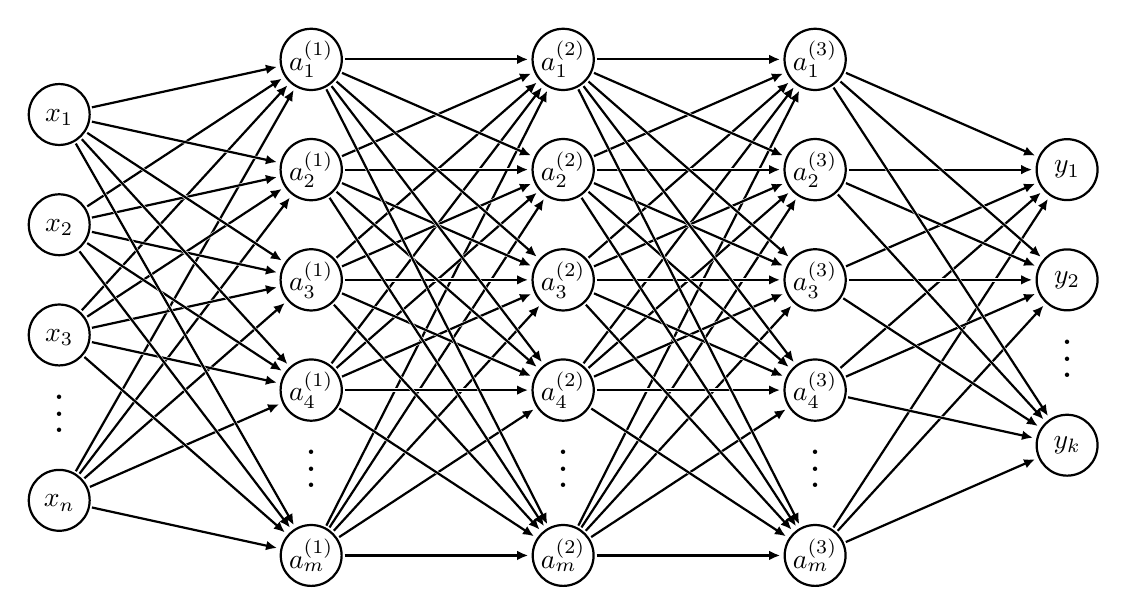
\begin{tikzpicture}[x=3.2cm,y=1.4cm]
    \message{^^JNeural network, shifted}
    \readlist\Nnod{4,5,5,5,3} % array of number of nodes per layer
    \readlist\Nstr{n,m,m,m,k} % array of string number of nodes per layer
    \readlist\Cstr{\strut x,a^{(\prev)},a^{(\prev)},a^{(\prev)},y} % array of coefficient symbol per layer
    \def\yshift{0.5} % shift last node for dots
    
    \message{^^J  Layer}
    \foreachitem \N \in \Nnod{ % loop over layers
      \def\lay{\Ncnt} % alias of index of current layer
      \pgfmathsetmacro\prev{int(\Ncnt-1)} % number of previous layer
      \message{\lay,}
      \foreach \i [evaluate={\c=int(\i==\N); \y=\N/2-\i-\c*\yshift;
                  \index=(\i<\N?int(\i):"\Nstr[\lay]");
                  \x=\lay; \n=\nstyle;}] in {1,...,\N}{ % loop over nodes
        % NODES
        \node[node \n] (N\lay-\i) at (\x,\y) {$\Cstr[\lay]_{\index}$};
        
        % CONNECTIONS
        \ifnum\lay>1 % connect to previous layer
          \foreach \j in {1,...,\Nnod[\prev]}{ % loop over nodes in previous layer
            \draw[connect,white,line width=1.2] (N\prev-\j) -- (N\lay-\i);
            \draw[connect arrow] (N\prev-\j) -- (N\lay-\i);
            %\draw[connect] (N\prev-\j.0) -- (N\lay-\i.180); % connect to left
          }
        \fi % else: nothing to connect first layer
        
      }
      \path (N\lay-\N) --++ (0,1+\yshift) node[midway,scale=1.5] {$\vdots$};
    }
    
  \end{tikzpicture}
  \caption{Schematic representation of a neural network.}
  \label{fig:nnschematic}
\end{figure}

% NEURAL NETWORK activation
% https://www.youtube.com/watch?v=aircAruvnKk&list=PLZHQObOWTQDNU6R1_67000Dx_ZCJB-3pi&index=1
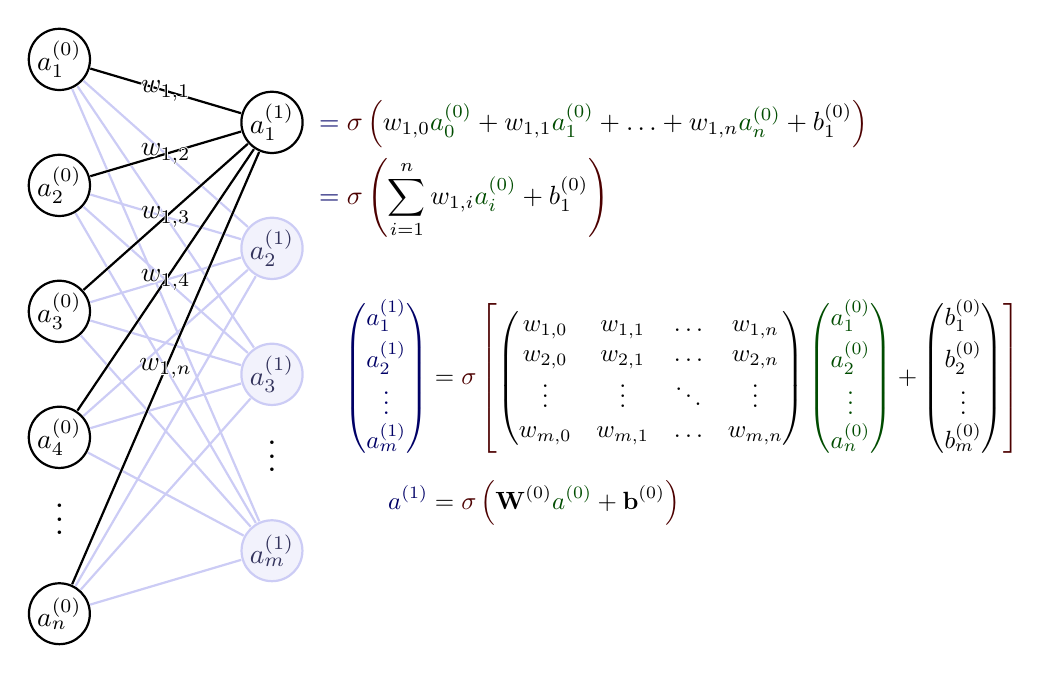
\begin{tikzpicture}[x=2.7cm,y=1.6cm]
  \message{^^JNeural network activation}
  \def\NI{5} % number of nodes in input layers
  \def\NO{4} % number of nodes in output layers
  \def\yshift{0.4} % shift last node for dots
  
  % INPUT LAYER
  \foreach \i [evaluate={\c=int(\i==\NI); \y=\NI/2-\i-\c*\yshift; \index=(\i<\NI?int(\i):"n");}]
              in {1,...,\NI}{ % loop over nodes
    \node[node in,outer sep=0.6] (NI-\i) at (0,\y) {$a_{\index}^{(0)}$};
  }
  
  % OUTPUT LAYER
  \foreach \i [evaluate={\c=int(\i==\NO); \y=\NO/2-\i-\c*\yshift; \index=(\i<\NO?int(\i):"m");}]
    in {\NO,...,1}{ % loop over nodes
    \ifnum\i=1 % high-lighted node
      \node[node hidden]
        (NO-\i) at (1,\y) {$a_{\index}^{(1)}$};
      \foreach \j [evaluate={\index=(\j<\NI?int(\j):"n");}] in {1,...,\NI}{ % loop over nodes in previous layer
        \draw[connect,white,line width=1.2] (NI-\j) -- (NO-\i);
        \draw[connect] (NI-\j) -- (NO-\i)
          node[pos=0.50] {\contour{white}{$w_{1,\index}$}};
      }
    \else % other light-colored nodes
      \node[node,blue!20!black!80,draw=myblue!20,fill=myblue!5]
        (NO-\i) at (1,\y) {$a_{\index}^{(1)}$};
      \foreach \j in {1,...,\NI}{ % loop over nodes in previous layer
        %\draw[connect,white,line width=1.2] (NI-\j) -- (NO-\i);
        \draw[connect,myblue!20] (NI-\j) -- (NO-\i);
      }
    \fi
  }
  
  % DOTS
  \path (NI-\NI) --++ (0,1+\yshift) node[midway,scale=1.2] {$\vdots$};
  \path (NO-\NO) --++ (0,1+\yshift) node[midway,scale=1.2] {$\vdots$};
  
  % EQUATIONS
  \def\agr#1{{\color{mydarkgreen}a_{#1}^{(0)}}}
  \node[below=17,right=11,mydarkblue,scale=0.95] at (NO-1)
    {$\begin{aligned} %\underset{\text{bias}}{b_1}
       &= \color{mydarkred}\sigma\left( \color{black}
            w_{1,0}\agr{0} + w_{1,1}\agr{1} + \ldots + w_{1,n}\agr{n} + b_1^{(0)}
          \color{mydarkred}\right)\\
       &= \color{mydarkred}\sigma\left( \color{black}
            \sum_{i=1}^{n} w_{1,i}\agr{i} + b_1^{(0)}
           \color{mydarkred}\right)
     \end{aligned}$};
  \node[right,scale=0.9] at (1.3,-1.3)
    {$\begin{aligned}
      {\color{mydarkblue}
      \begin{pmatrix}
        a_{1}^{(1)} \\[0.3em]
        a_{2}^{(1)} \\
        \vdots \\
        a_{m}^{(1)}
      \end{pmatrix}}
      &=
      \color{mydarkred}\sigma\left[ \color{black}
      \begin{pmatrix}
        w_{1,0} & w_{1,1} & \ldots & w_{1,n} \\
        w_{2,0} & w_{2,1} & \ldots & w_{2,n} \\
        \vdots  & \vdots  & \ddots & \vdots  \\
        w_{m,0} & w_{m,1} & \ldots & w_{m,n}
      \end{pmatrix}
      {\color{mydarkgreen}
      \begin{pmatrix}
        a_{1}^{(0)} \\[0.3em]
        a_{2}^{(0)} \\
        \vdots \\
        a_{n}^{(0)}
      \end{pmatrix}}
      +
      \begin{pmatrix}
        b_{1}^{(0)} \\[0.3em]
        b_{2}^{(0)} \\
        \vdots \\
        b_{m}^{(0)}
      \end{pmatrix}
      \color{mydarkred}\right]\\[0.5em]
      {\color{mydarkblue}a^{(1)}}
      &= \color{mydarkred}\sigma\left( \color{black}
           \mathbf{W}^{(0)} {\color{mydarkgreen}a^{(0)}}+\mathbf{b}^{(0)}
         \color{mydarkred}\right)
         %\color{black},\quad \mathbf{W}^{(0)} \in \mathbb{R}^{m\times n}
    \end{aligned}$};
  
\end{tikzpicture}

\bibliographystyle{JHEP}
\bibliography{bib}
\end{document}
